\documentclass[11pt]{article}

\usepackage{geometry}
% make full use of A4 papers
\geometry{margin=1.5cm, vmargin={0pt,1cm}}
\setlength{\topmargin}{-1cm}
\setlength{\paperheight}{29.7cm}
\setlength{\textheight}{25.1cm}
\usepackage[BoldFont,SlantFont,CJKchecksingle]{xeCJK}%CJKsetspaces
\setCJKmainfont[BoldFont=SimHei]{SimSun}
\setCJKmonofont{SimSun}% 设置缺省中文字体
\parindent 2em   %段首缩进

\usepackage{setspace}
% \setlength{\baselineskip}{25pt}
\linespread{1.25}
% auto adjust the marginals
\usepackage{marginfix}
\usepackage{amsfonts}
\usepackage{amsmath}
\usepackage{amssymb}
\usepackage{amsthm}
\usepackage{CJKutf8}   % for Chinese characters
\usepackage{enumerate}
\usepackage{fancyhdr}
\usepackage{graphicx}  % for figures
\usepackage{layout}
\usepackage{mathrsfs}  
\usepackage{multicol}  % multiple columns to reduce number of pages
%\usepackage{natbib}
\usepackage{subfigure}
\usepackage{tcolorbox}
\usepackage{tikz-cd}
\usepackage{extarrows}
\usepackage{float}

\usepackage[backend=biber,style=gb7714-2015]{biblatex}
\addbibresource[location=local]{bib/3Dmars.bib}

%------------------
% common commands %
%------------------
% differentiation
\newcommand{\aff}{\mathrm{aff}}
\newcommand{\conv}{\mathrm{conv}}
\newcommand{\VertSet}{\mathrm{Vert}}
\newcommand{\Star}{\mathrm{st}}
\newcommand{\gen}[1]{\left\langle #1 \right\rangle}
\newcommand{\dif}{\mathrm{d}}
\newcommand{\difPx}[1]{\frac{\partial #1}{\partial x}}
\newcommand{\difPy}[1]{\frac{\partial #1}{\partial y}}
\newcommand{\Dim}{\mathrm{D}}
\newcommand{\avg}[1]{\left\langle #1 \right\rangle}
\newcommand{\sgn}{\mathrm{sgn}}
\newcommand{\Span}{\mathrm{span}}
\newcommand{\dom}{\mathrm{dom}}
\newcommand{\Arity}{\mathrm{arity}}
\newcommand{\Int}{\mathrm{Int}}
\newcommand{\Ext}{\mathrm{Ext}}
\newcommand{\Cl}{\mathrm{Cl}}
\newcommand{\Fr}{\mathrm{Fr}}
% group is generated by
\newcommand{\grb}[1]{\left\langle #1 \right\rangle}
% rank
\newcommand{\rank}{\mathrm{rank}}
\newcommand{\Iden}{\mathrm{Id}}
\newcommand{\Obj}[1]{\mathrm{obj}\,{\mathscr #1}}
\newcommand{\Hom}{\mathrm{Hom}}

% this environment is for solutions of examples and exercises
\newenvironment{solution}%
{\noindent\textbf{Solution.}}%
{\qedhere}

%the following command is for disabling environments
%  so that their contents do not show up in the pdf.
\makeatletter
\newcommand{\voidenvironment}[1]{%
  \expandafter\providecommand\csname env@#1@save@env\endcsname{}%
  \expandafter\providecommand\csname env@#1@process\endcsname{}%
  \@ifundefined{#1}{}{\RenewEnviron{#1}{}}%
}
\makeatother

%---------------------------------------------
% commands specifically for complex analysis %
%---------------------------------------------
% complex conjugate
\newcommand{\ccg}[1]{\overline{#1}}
% the imaginary unit
\newcommand{\ii}{\mathbf{i}}
%\newcommand{\ii}{\boldsymbol{i}}
% the real part
\newcommand{\Rez}{\mathrm{Re}\,}
% the imaginary part
\newcommand{\Imz}{\mathrm{Im}\,}
% punctured complex plane
\newcommand{\pcp}{\mathbb{C}^{\bullet}}
% the principle branch of the logarithm
\newcommand{\Log}{\mathrm{Log}}
% the principle value of a nonzero complex number
\newcommand{\Arg}{\mathrm{Arg}}
\newcommand{\Null}{\mathrm{null}\,}
\newcommand{\Range}{\mathrm{range}\,}
\newcommand{\Ker}{\mathrm{ker}}
\newcommand{\Iso}{\mathrm{Iso}}
\newcommand{\Aut}{\mathrm{Aut}}
\newcommand{\ord}{\mathrm{ord}}
\newcommand{\Res}{\mathrm{Res}}
%\newcommand{\GL2R}{\mathrm{GL}(2,\mathbb{R})}
\newcommand{\GL}{\mathrm{GL}}
\newcommand{\SL}{\mathrm{SL}}
\newcommand{\Dist}[2]{\left|{#1}-{#2}\right|}



%----------------------------------------
% theorem and theorem-like environments %
%----------------------------------------
% \numberwithin{equation}{chapter}
% \theoremstyle{definition}

% \newtheorem{thm}{Theorem}[chapter]
% \newtheorem{axm}[thm]{Axiom}
% \newtheorem{alg}[thm]{Algorithm}
% \newtheorem{asm}[thm]{Assumption}
% \newtheorem{defn}[thm]{Definition}
% \newtheorem{frm}[thm]{Formula}
% \newtheorem{prop}[thm]{Proposition}
% \newtheorem{qst}[thm]{Question}
% \newtheorem{rul}[thm]{Rule}
% \newtheorem{coro}[thm]{Corollary}
% \newtheorem{lem}[thm]{Lemma}
% \newtheorem{exm}{Example}[chapter]
% \newtheorem{rem}{Remark}[chapter]
% \newtheorem{exc}[exm]{Exercise}
% \newtheorem{ntn}{Notation}


%----------------------
% the end of preamble %
% ----------------------


\begin{document}
% \begin{CJK*}{UTF8}{gkai}
% 		\CJKindent
 % \makeatletter %将文献引用作为上标出现,增加括号,
 % \def\@cite#1#2{\textsuperscript{[{#1\if@tempswa , #2\fi}]}}

 % \makeatother
 \theoremstyle{definition}%amsthm 宏包 标签正体,内容正体
 \newtheorem{thm}{{定理}}
 \newtheorem{lem}[thm]{{引理}}
 \newtheorem{defn}[thm]{{定义}}
\newtheorem{prop}[thm]{{性质}}
 \newtheorem{cor}[thm]{{推论}}
 \newtheorem{nota}[thm]{{记号}}
 \newtheorem{exm}{{例}}
 \newtheorem{rem}[exm]{{注}}
 \newtheorem*{pro}{证明}

\title{三维高阶界面追踪}
\author{应林洁,李祎玲,金鹏炜}
\date{}
\maketitle


\section{界面追踪问题}
利用殷空间\cite{zhang2018fourth}的概念描述界面追踪问题。
\begin{defn}[界面追踪问题]
  \label{IT}
  用一个殷集$\mathcal{M}(t) \in \mathbb{Y}$表示被追踪物质$M$在$t$时刻所处区域,
  由初始条件$\mathcal{M}(t_0)$和给定流速场$\boldsymbol{u}(\boldsymbol{x},t)(t\in [t_0,T])$
  确定$\mathcal{M}(T)$的问题称为界面追踪问题。
\end{defn}
为了度量界面追踪的精度,利用\cite{zhang2018fourth}中度量(2.10)定义误差
\begin{equation}
  \label{eq:geomError}
  E_1(t_n) := \|\mathcal{M}(t_n) \oplus
  \mathcal{M}^{n}\| = \sum_{{\mathcal C}\subset \Omega}
  \left\|\mathcal{M}_{\mathcal C}(t_n) \oplus
    \mathcal{M}_{\mathcal C}^{n}\right\|,
\end{equation}
其中,$\mathcal{M}(t_n)$表示$t_n$时刻精确流体区域,
$\mathcal{M}^{n}$是$\mathcal{M}(t_n)$的一个近似,
所有控制体$\mathcal{C}$的集合形成计算域$\Omega$的一个划分。

\begin{defn}[界面追踪方法的精度]
  数值求解界面追踪问题(定义\ref{IT}),称一个界面追踪方法$\mathcal{L}_{IT}$
  \begin{equation}
    \label{eq:ITM}
    \mathcal{M}^{n+1}=\mathcal{L}_{IT}(\mathcal{M}(t_n),\boldsymbol{u})\approx \mathcal{M}(t_{n+1}),
  \end{equation}
  在$1-$范数下有$\beta$阶精度,若
  \begin{displaymath}
    E_1(T) = O(k^{\beta})(k \to 0).
  \end{displaymath}
  称$\mathcal{L}_{IT}$是一致的,若$\beta > 0$.
\end{defn}



\section{MARS方法\cite{zhang2016mars}}

在界面追踪(IT)问题当中,我们通常得到一个先验的速度场
$\mathbf{u}(\mathbf{x},t),$
每个流体相通过这个速度场推进,对应的常微分方程如下:
\begin{equation}
\label{volEquation}
\frac{\mathrm{d}\, \mathbf{x}}{\mathrm{d}\, t}=\mathbf{u}(\mathbf{x},t),
\end{equation}
若速度场$\mathbf{u}(\mathbf{x},t)$对时间$t$连续,
在空间$\mathbb{R}^{\textup{D}}$上Lipschitz连续,
则其存在唯一解。由解的唯一性可得流映射 $\phi: \mathbb{R}^{\textup{D}}\times \mathbb{R}\times\mathbb{R}\rightarrow \mathbb{R}^{\text{D}}$.
\begin{equation} 
\label{eq:tracing}
\renewcommand{\arraystretch}{1.3}
\left\{
\begin{array}{l}
\phi_{t_0}^{+k}(p) := p(t_0+k) 
= p(t_0) + \int_{t_0}^{t_0+k} \mathbf{u}(p(t),t)\,\mathrm{d}\, t,
\\
\phi_{t_0}^{-k}(p) := p(t_0-k) 
= p(t_0) + \int_{t_0}^{t_0-k} \mathbf{u}(p(t),t)\,\mathrm{d}\,t.
\end{array}
\right.
\end{equation}
将流映射推广到任意点集有:
\begin{displaymath}
\phi_{t_0}^{\pm k}({\mathcal M})  
= \{\phi_{t_0}^{\pm k}(p) : p\in {\mathcal M}\}.
\end{displaymath}
% 记 $\overleftarrow{M}:=\phi_{t_0+k}^{-k}(M)$, $\overrightarrow{M}:=\phi_{t_0}^{+k}(M)$, 
% 其中$t_0$表示当前时刻,$k$表示时间步间隔。

\begin{defn}
	一个半离散流映射$\mathring{ \phi} : \mathbb{S}^{\textup{D}}\rightarrow \mathbb{S}^{\textup{D}}$
	是用一个一致的时间积分方法求解\eqref{volEquation}式得到的精确流映射$\phi$的近似.
	称$\mathring{ \phi}_{t_0}^{nk}$在时间上是$\kappa$阶精度的,
	若对于任意的$p(t_0)\in \mathbb{R}^{\textup{D}}$, $t_0+nk\leq T$,
	有$\mathring{ \phi}_{t_0}^{nk}=\phi_{t_0}^{nk}(p)+O(k^{\kappa})$.
\end{defn}
\begin{defn}
	一个离散流映射$\varphi : \mathbb{S}_q^{\textup{D}}\rightarrow\mathbb{S}_q^{\textup{D}}$
	是半离散流映射$\mathring{ \phi}$的近似,由以下两步所得,
	\begin{enumerate}
		\item 把$\mathring{ \phi}$作用到边界$\mathcal{P}$的顶点($0$-单形)上;
		\item 构造一个$\mathring{ \phi}(\partial\mathcal{P})$的多项式与$\partial \mathcal{P}$同胚。
		当$q=1$时,在二维情况下,边界由相连的直线近似;
		在三维情况下,边界由多个三角平面组成的多面体来近似。
	\end{enumerate}
\end{defn}

\begin{defn}
	\label{defn:MARS}
	MARS方法是具有以下形式的界面追踪方法
	\begin{equation*}
	\label{eq:interfaceTrackingMethod}
	{\mathcal M}^{n+1}={\mathfrak L}_{\mathrm{Mars}}^n {\mathcal M}^n
	:= \left(\chi_{n+1}\circ\varphi_{t_n}^k\circ\psi_n
	\right){\mathcal M}^n,
	\end{equation*}
	其中$\mathcal{M}^n\in\mathbb{Y}$ 是$\mathcal{M}(t_n)\in\mathbb{Y}$的近似,
	$\varphi:\mathbb{Y}\rightarrow
	\mathbb{Y}$ 是\eqref{eq:tracing}式中$\phi$的离散流映射, 
	$\psi_n:\mathbb{Y}\rightarrow \mathbb{Y}$是预处理算子,
	$\chi_{n+1}:\mathbb{Y}\rightarrow \mathbb{Y}$是后处理算子。
\end{defn}

\begin{defn}
  考虑一种MARS方法,
  其中映射操作$\varphi$根据精确的映射$\phi$
  在时间上离散化后得到$\mathring{ \phi}$,
  再在空间上离散$\mathring{ \phi}$得到。
  MARS方法在$t_n=t_0+nk$时刻的
  时间积分误差$E^{\mathrm{ODE}}(t_n),$
  表示误差$E^{\mathrm{REP}}(t_n),$
  扩充误差$E^{\mathrm{AUG}}(t_n),$
  映射误差$E^{\mathrm{MAP}}(t_n),$
  以及调整误差$E^{\mathrm{ADJ}}(t_n)$分别如下:
  \begin{equation}\label{defn:error}
    \left\{
      \begin{array}{rl}
	E^{\mathrm{ODE}}(t_n) &:= \| \phi_{t_0}^{nk}(\mathcal{M}^0) \oplus \mathring{ \phi}_{t_0}^{nk}(\mathcal{M}^0) \|;\\[0.2cm]
	E^{\mathrm{REP}}(t_n) &:= \| \phi_{t_0}^{nk}(\mathcal{M}(t_0)) \oplus  \phi_{t_0}^{nk}(\mathcal{M}^0) \|;\\[0.2cm]
	\varepsilon_i^{\mathrm{AUG}} &:=  ( \psi_i \mathcal{M}^i )\oplus \mathcal{M}^i, \\[0.2cm]
	E^{\mathrm{AUG}}(t_n) &:= \| \oplus_{j=0}^{n-1} \mathring{ \phi}_{t_j}^{(n-j)k}\varepsilon_j^{\mathrm{AUG}} \|;\\[0.2cm]
	\varepsilon_i^{\mathrm{MAP}}(t_n)& := \mathring{ \phi}_{t_i}^k(\psi_i\mathcal{M}^i)\oplus \varphi_{t_i}^k(\psi_i\mathcal{M}^i),\\[0.2cm]
	E^{\mathrm{MAP}}(t_n) &:=  \| \oplus_{j=1}^n \mathring{ \phi}_{t_j}^{(n-j)k}\varepsilon_{j-1}^{\mathrm{MAP}} \|;\\[0.2cm]
	\varepsilon_{i+1}^{\mathrm{ADJ}} &:= (\varphi_{t_i}^k\psi_i\mathcal{M}^i)\oplus\mathcal{M}^{i+1},\\[0.2cm]
	E^{\mathrm{ADJ}}(t_n) &:= \| \oplus_{j=1}^n\mathring{ \phi}_{t_j}^{(n-j)k}\varepsilon_j^{\mathrm{ADJ}}\|.\\[0.2cm]
      \end{array}\right.
  \end{equation}
  $\varepsilon_i^{\mathrm{AUG}}$, $\varepsilon_i^{\mathrm{MAP}}$, $\varepsilon_{i+1}^{\mathrm{ADJ}}$称为第$i$个时间步的误差区域。
\end{defn}
这里$E^{\mathrm{ODE}}$是用半离散流映射$\mathring{ \phi}$近似精确流映射$\phi$造成的误差,
$E^{\mathrm{REP}}$是在初始时刻用半代数集表示流相的误差,
$E^{\mathrm{AUG}}$是扩充半代数集的累计误差,
$E^{\mathrm{MAP}}$是用映射操作近似半离散流映射的累计误差,
$E^{\mathrm{ADJ}}$是调整半代数集的像的累计误差。

\begin{thm}
定义\ref{defn:MARS}中的MARS方法是殷空间上的三个算子的复合,
通过\eqref{defn:error}式定义的各类单一误差以及对每个算子的分析,
得MARS方法的整体误差满足:
 \begin{equation}
\label{eq:E1parts}
E_1(t_n)  \le E^{\mathrm{ODE}} + E^{\mathrm{MAP}}
+ E^{\mathrm{REP}} + E^{\mathrm{AUG}} + E^{\mathrm{ADJ}}.
\end{equation}
这里的 $E^{\mathrm{ODE}},$$E^{\mathrm{MAP}},$
$E^{\mathrm{REP}},$ $E^{\mathrm{AUG}},$$E^{\mathrm{ADJ}}$
均由\eqref{defn:error}给出。
\end{thm}

\begin{pro}
  见\cite{zhang2016mars}. 
\end{pro}

\begin{prop}
  \label{ODEerror}
  如果一个MARS方法的半离散流映射$\mathring{ \phi}$有$\kappa$阶精度,
  则对任意$t_n = t_0 + nk(k = O(\frac{1}{n}))$有
  \begin{displaymath}
    E^{\rm{ODE}}(t_n) = O(k^{\kappa}).
  \end{displaymath}
\end{prop}
\begin{pro}
  见\cite{zhang2016mars}.
\end{pro}

\section{算法}
\label{sec:algorithm}

%\begin{verbatim}
%分析
%\end{verbatim}

\begin{defn}[三维界面追踪的高阶MARS方法]\label{defn:algorithm}
  令相邻示踪点的距离范围为$[r_\textmd{tiny}h_L,h_L].$
在每一个时间步$[t_n,t_n+k]$中,
三维界面追踪的高阶MARS方法
以$t_n$时刻殷集边界$\partial {\cal M}(t_n)$
的一组近似曲面片作为输入,
通过以下步骤得到对$\partial {\cal M}(t_n+k)$近似
的一组三次多项式曲面片$\partial {\cal M}^{n+1}$
作为界面追踪结果:
  \begin{enumerate}[{(SplineMARS}-1)]
    \setlength{\itemsep}{0pt} \setlength{\parsep}{0pt}
    \setlength{\parskip}{0pt}
  \item
    对$\partial\mathcal{M}(t_n)$上的示踪点,由流速场$\mathbf{u}$得到这些
    示踪点在$t_n+k$时刻的位置,记为$\{p_j\}$.
  \item 检查每一个三角形,若$\triangle_{p_i p_j p_k}$存在一条或一条以上
    的边大于上界$h_L$, 
    \begin{enumerate}[(a)]
    \item
      在$\partial\mathcal{M}^n$上定位
      $\triangle_{p_i p_j p_k}$的顶点原像
      $\overleftarrow{p_i},\overleftarrow{p_j},\overleftarrow{p_k}$,
    \item  将三角形$\triangle_{\overleftarrow{p_i}
        \overleftarrow{p_j}\overleftarrow{p_k}}$中
      大于上界$h_L$的边等分为
      $\lceil\frac{\lVert p_j-p_{j+1}\rVert_2}{h_L}\rceil $段,
      计算输入的$\partial\mathcal{M}^n$曲面片上的对应点
      并标记为新的示踪点,
    \item  将$\overleftarrow{p_i}, \overleftarrow{p_j}, 
      \overleftarrow{p_k}$的star上的点
      以及新的示踪点投影在三角形平面上,
      构建一个新的局部三角剖分,
    \item 将新的局部三角剖分关系更新到整体的三角剖分网格中,
    \item
      由流速场$\mathbf{u}$
     % 求解常微分方程$\frac{\text{d}\mathbf{x}}{\text{d}t}=\mathbf{u}$
      得到这些新的示踪点在$t_n+k$时刻的位置并加入到顶点序列$\{p_j\}$中。
    \end{enumerate}
    重复以上步骤直到所有三角形边长都不大于上界$h_L$。
  \item 检查每个三角形,若$\triangle_{p_i p_j p_k}$的面积小
    于$\frac{r_{\textmd{tiny}} \cdot h_L^2}{2}$:
    \begin{enumerate}
    \item
      若三角形$\triangle_{p_i p_j p_k}$中有两条或以上的边小
      于$r_\textmd{tiny}h_L$, 将该三角形缩成一个点;
    \item
      若三角形$\triangle_{p_i p_j p_k}$仅有一边小
      于$r_\textmd{tiny}h_L$,将该边缩成一个点;
    \item
      若三角形$\triangle_{p_i p_j p_k}$三条边都符合标准,用换边法优化网
      格,若无法优化则将三角形的最小边缩成一个点。
    \end{enumerate}
  \item 得到一个新的三角剖分信息,用这个三角剖分构造一个新的曲面。
  \item (可选)若需要可视化曲面,
    用三角剖分信息构造全局光滑的曲面作为输出。
  \end{enumerate}
\end{defn}

\begin{rem}
  在上述算法中,$h_L$和$r_{\textmd{tiny}}$都是由用户指定的,$h_L$为界面
  追踪的物理尺度。为了避免示踪点数量的无限增长,指
  定$r_{\textmd{tiny}}h_L$和$\frac{r_{\textmd{tiny}} \cdot h_L^2}{2}$分
  别为示踪点距离和面积的下界。由于相邻点过近时的计算几何中的鲁棒性问题%看文章
  $r_{\textmd{tiny}}$不能过小;为了防止频繁加减点导致的计算效率下
  降,$r_{\textmd{tiny}}$不能过大。
\end{rem}


\begin{figure}[H]
  \centering
  \subfigure[$\mathcal{M}^n$边界上示踪点向前移动一个时间步.]{
    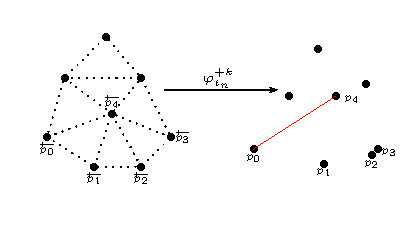
\includegraphics[width=0.45\linewidth]{pst/perform1}
  }
  \hfill
  \subfigure[通过在$\mathcal{M}^n$边界上增加示踪点确保$\mathcal{M}^{n+1}$边界上相邻示踪点的距离不超过上界$h_L$.]{
    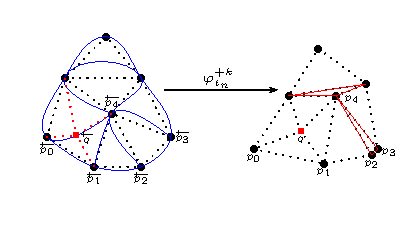
\includegraphics[width=0.45\linewidth]{pst/perform2}
  }
  \hfill
  \subfigure[通过换边优化确保$\mathcal{M}^{n+1}$边界的三角剖分中三角形的面积不低于下界$\frac{r_{\rm{tiny}}h_{L}^2}{2}$.]{
    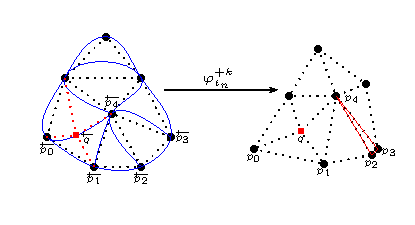
\includegraphics[width=0.45\linewidth]{pst/perform3}
  }
  \hfill
  \subfigure[通过将边或三角形缩为一点确保$\mathcal{M}^{n+1}$边界的三角剖分中三角形的面积不低于下界$\frac{r_{\rm{tiny}}h_{L}^2}{2}$且相邻示踪点的距离不低于下界$r_{\rm{tiny}}h_L$.]{
    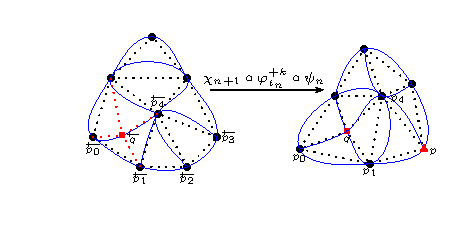
\includegraphics[width=0.5\linewidth]{pst/perform4}
  }
  \label{fig:algorithm}
\end{figure}


\begin{rem}
  在近似殷集边界$\partial {\cal M}(t_n)$
  的一组在顶点$C^0$连续,
  在三角形边界不连续的三次三角曲面片中,
  每一个三角剖分的三角形边对应两个不同三角曲面片边界,
  即两条空间三次曲线
  $\vec{\gamma}_1(t),\vec{\gamma}_2(t)
  : \mathbb{R}^1\rightarrow \mathbb{R}^3,
  0\leq t\leq 1.$
  将两条曲线对应的点$\vec{\gamma}_1(t_0),\vec{\gamma}_2(t_0)$
  用直线段连接,
  直线段上一点$\vec{p}$可以用参数表示为
  \begin{displaymath}
    \vec{p}(s)=(1-s)\vec{\gamma}_1(t_0)+s\vec{\gamma}_2(t_0)
    \quad s\in [0,1].
  \end{displaymath}
  因此两个相邻曲面片连接处的曲面可以表示为二元四次的多项式向量函数
    \begin{displaymath}
    \vec{p}(t,s)=(1-s)\vec{\gamma}_1(t)+s\vec{\gamma}_2(t)
    \quad s,t\in [0,1].
  \end{displaymath}
  三维四阶MARS算法中的离散流映射
  $\mathring{\varphi}:\mathbb{S}^3_4\rightarrow \mathbb{S}^3_4 $。
  其中离散流映射作用的半代数集合${\cal P}\in \mathbb{S}^3_4$
  的边界$\partial {\cal P}$是由一组二元三次三角面片
  以及连接三角曲面片的的二元四次曲面构成的闭合$C^0$曲面。
\end{rem}

\begin{figure}[H]
    \centering
    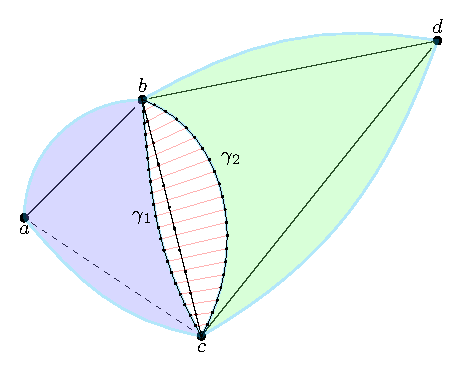
\includegraphics[width=0.3\linewidth]{tikz/connectSurface}
    \label{fig:connect}
  \end{figure}

\begin{rem}
  注意到$t_n+k$时刻同一个三角面片构造所用的插值点不一定是
  $t_n$时刻对应的点映射所得到的。
  我们可以把算法中(MSRS-2)所对应的在$t_n$时刻加示踪点的操作
  视为预处理(augment)算子$\psi_n$,
  把$t_{n+1}$时刻算法中(MSRS-3)减去示踪点,
  和寻找构造曲面片所用的插值点的操作视为调整(adjustment)算子$\chi.$
  考虑MARS方法$t_{n+1}$时刻前的映射
  \begin{equation}
    \widetilde{{\cal M}}^n\stackrel{\chi}{\longrightarrow}
    {\cal M}^n\xlongrightarrow{\varphi_{t_n}^k\circ\psi_n}
    \widetilde{{\cal M}}^{n+1}\xlongrightarrow{\chi}{\cal M}^{n+1}.
  \end{equation}
  其中$\partial\widetilde{{\cal M}}^{n+1}$的三角曲面片所用的
  拟合节点是由$\partial {\cal M}^n$上对应节点映射得到的。
\end{rem}
\subsection{误差分析}
\begin{rem}
  下面假定界面在光滑流场$\mathbf{u}$的作用下不会产生$C^1$不连续点。
\end{rem}

\begin{thm}\cite{zhang2016mars}[MARS误差控制]
  MARS框架下的界面追踪误差由下式控制:
   \begin{equation}
    E_1(t_n)\leq E^{AUG}+E^{ADJ}+E^{MAP}+E^{REP}+E^{ODE}.
  \end{equation}
\end{thm}

\begin{prop}
  $\kappa$阶精度的半离散流映射$\mathring{\phi}$满足
  \begin{equation}
    \label{eq:1}
    \forall {\cal P} \in \mathbb{S}^3,\quad
    \lVert \mathring{\phi}^k_{t_n}({\cal P})\oplus
    \phi^k_{t_n}({\cal P})\rVert \leq O(k^{\kappa +1}).
  \end{equation}
\end{prop}
\begin{pro}
  见[MARS]\cite{zhang2016mars}性质3.6。
\end{pro}

\subsubsection{映射误差$E^{\textmd{MAP}}$}
\label{sec:拟合误差}



\begin{lem}\label{lem:maperror}
  用离散流映射$\varphi:\mathbb{S}^3_4(\triangle)\rightarrow
 \mathbb{S}^3_4(\triangle)$逼近半离散流映射$\mathring{\phi}$.
 若流速场光滑,
 $\mathring{\phi}$是$\kappa$阶精度的。
  则对任意的${\cal P}\in \mathbb{S}^3_4$,有
  \begin{equation}\label{equ:dis-semi}
    \lVert \varphi^k_{t_n}({\cal P})\oplus
    \mathring{\phi}^k_{t_n}({\cal P})\rVert
    \leq O(kh^4_{L,{\cal P}}+k^{\kappa +1}).
  \end{equation}
\end{lem}

\begin{pro}
  对三角剖分$\triangle$中三角形$T$,
  令点$p $是$T$中一点对应
  的$ \partial {\cal P}$上的一个点。
  对$t_n+k$时刻三角形$T$三个顶点
  $\phi^k_{t_n}(p_1),\phi^k_{t_n}(p_2),
  \phi^k_{t_n}(p_3)$插值、
  对点$\phi^k_{t_n}(p_4),...,\phi^k_{t_n}(p_M)$
  插值或最小二乘拟合得到的近似曲面
  $\vec{f}(\mathbf{x})=\sum_{i=1}^{N}
  (\sum_{j=1}^Mb_{ij}\phi^k_{t_n}(p_j))B_i(\mathbf{x}).$
  其中对三次样条基函数有$N=10,M\geq N.$
  由数值实验知,
  曲面片$\vec{f}(p)$对光滑曲面的拟合有四阶精度,
  即,设$\vec{g}(p)$是任意经过点$p_1,...,p_N$
  的光滑曲面,%C^3连续?需要测试
  则$\lVert \vec{g}(p)-\vec{f}(p)\rVert =O(h_L^4).$
  \begin{equation}
    \label{eq:2}
    \begin{aligned}
   \left\lVert\varphi^k_{t_n}(p)-\mathring{\phi}^k_{t_n}(p)
     \right\rVert &=\left\lVert
     \sum_{j=1}^M\left(\sum_{i=1}^{N}
       b_{ij}B_i\left(\varphi^k_{t_n}(p)\right)\right)
     \mathring{\phi}^k_{t_n}(p_j)
    -\mathring{\phi}^k_{t_n}(p) \right\rVert\\
    &=\left\lVert
      \sum_{j=1}^M\left(\sum_{i=1}^{N}b_{ij}B_i
        \left(\varphi^k_{t_n}(p)\right)\right)
      \phi^k_{t_n}(p_j)-\phi^k_{t_n}(p)\right\rVert
    +O(k^{\kappa+1})\\
    &=\left\lVert
      \vec{f}(\varphi^k_{t_n}(p))-\phi^k_{t_n}(p)\right\rVert
    +O(k^{\kappa+1})\\
    &=O(h_L^4)+O(k^{\kappa+1}).
  \end{aligned}
\end{equation}
又因为对于给定的$h_L$,由$\mathring{\phi}$和$B_i$的连续性有
$$\lim_{k\rightarrow 0}\left\lVert
  \varphi^k_{t_n}(p)-\mathring{\phi}^k_{t_n}(p)
\right\rVert = \left\lVert
  \sum_{i=1}^{N}(\sum_{j=1}^Mb_{ij}p_j)B_i(p)-p\right\rVert=0.$$
所以误差$\left\lVert \varphi^k_{t_n}(p)
-\mathring{\phi}^k_{t_n}(p)\right\rVert$
或者$\left\lVert
      \vec{f}(\phi^k_{t_n}(p))-\phi^k_{t_n}(p)\right\rVert$
必然是时间相关的。
又
\begin{equation}\label{eq:k}
  \vec{f}(\phi^k_{t_n}(p))-\phi^k_{t_n}(p)
    =\sum_{i=1}^{N}\tilde{c}_iB_i\left(\varphi^k_{t_n}(p)\right)
    -p+p-\phi^k_{t_n}(p)
    = \sum_{i=1}^{N}\tilde{c}_iB_i\left(p\right) -\sum_{i=1}^{N}c_iB_i(p)
    +p-\phi^k_{t_n}(p).
\end{equation}
其中,第一个等式中$\tilde{c}_i=\sum_{j=1}^{M}b_{ij}\phi^k_{t_n}(p_j),$
第二个等号后面$c_i$是$t_n$时刻$\partial {\cal P}$的局部插值系数,
即对$p_1,p_2,\ldots,p_M$插值的三次曲面的插值基函数系数。
第二个等式中假定映射之后点$\varphi^k_{t_n}(p)$
在投影平面上的三角形重心坐标和映射之前的$p$重心坐标相同。
又由中值定理得到
\begin{equation}\label{equ:timeError}
  \left\lVert \phi^k_{t_n}(p)-p\right\rVert
  = \left\lVert \int_{t_0}^{t_0+k}
    \frac{\partial \phi}{\partial \tau}\textmd{d}\tau\right\rVert
  =O(k).
\end{equation}
定义
\begin{equation}
    \widetilde{\mathbf{B}}:=\left[B_1(\phi^k_{t_n}(p_j)),\ldots,B_N(\phi^k_{t_n}(p_j))\right]_{j=1}^{M},\quad
  \mathbf{B}:=\left[B_1(p_j),\ldots,B_N(p_j)\right]_{j=1}^{M}.
\end{equation}
由类似式子(\ref{equ:timeError})中关系,
$\phi^k_{t_n}(p_j)$的三角形重心坐标和$p_j$的重心坐标也有$O(k)$的误差。
根据基函数$B_j$的定义,
可以把矩阵$ \widetilde{\mathbf{B}}$表示为$\mathbf{B}+O(k)\mathbf{D}.$
定义
\begin{equation}
  \mathbf{c}=\left[c_1,\ldots,c_N\right]^{T},\quad
  \widetilde{\mathbf{c}}=\left[\widetilde{c}_1,\ldots,
    \widetilde{c}_N\right]^{T};\quad
  \mathbf{p}=\left[p_1,\ldots,p_M\right]^{T},\quad
\widetilde{\mathbf{p}}=\left[\phi^k_{t_n}(p_1),\ldots,
    \phi^k_{t_n}(p_M)\right]^{T}.
\end{equation}
则可以得到$\widetilde{\mathbf{p}}= \mathbf{p}+O(k)\mathbf{e}$,
$\widetilde{\mathbf{B}}\widetilde{\mathbf{c}}=\widetilde{\mathbf{p}}$,
$\mathbf{B}\mathbf{c}=\mathbf{p}.$
由于
\begin{displaymath}
  \begin{aligned}
    \left[\mathbf{B}+O(k)\mathbf{D}\right]   \widetilde{\mathbf{c}}
    &=\mathbf{p}+O(k)\mathbf{e}\Rightarrow
    \left[\mathbf{I}+O(k)\mathbf{B}^{-1}\mathbf{D}\right]
    \widetilde{\mathbf{c}}=\mathbf{c}+O(k) \mathbf{B}^{-1}\mathbf{e}
    \Rightarrow \widetilde{\mathbf{c}}-\mathbf{c}
    =O(k)\left(\mathbf{B}^{-1}\mathbf{e}-
      \mathbf{B}^{-1}\mathbf{D}\mathbf{\widetilde{c}}\right),\\
  \end{aligned}
\end{displaymath}
我们有$\left\lVert\sum_{i=1}^{N}\tilde{c}_iB_i\left(p\right)
  -\sum_{i=1}^{N}c_iB_i(p)\right\rVert=O(k),$
注意其中如果$M>N$则在等式两边同时乘以$B^T,$
用$(B^TB)^{-1}$即可($B$列满秩)。
因此误差精度可以被提高为
\begin{equation}
 \left\lVert\varphi^k_{t_n}(p)-\mathring{\phi}^k_{t_n}(p)
     \right\rVert=O(kh_K^4)+O(k^{\kappa+1}).
   \end{equation}
由积分中值定理和下面关系
\begin{equation}
  \label{eq:constant}
\lVert \partial {\cal P}\rVert = O(\lVert {\cal P}\rVert )
\end{equation}
可得(\ref{equ:dis-semi}).
\end{pro}

\begin{prop}\label{lem:e_map}
  $E^{\textmd{MAP}}(t_n)=O(h_L^4+k^\kappa)$.
\end{prop}
\begin{pro}
根据引理\ref{lem:maperror}和下面的式子(参见(4.17)[MARS])
\begin{equation}
  E^{\textmd{MAP}}(t_n)\leq c_k\sum_{j=1}^{n}\left\lVert
    {\cal E}^\textmd{MAP}_{j-1}\right \rVert.
\end{equation}
其中$n=O\left(\frac{1}{k}\right),c_k=O(1).$
  
\end{pro}

\subsubsection{后处理误差$E^{\textmd{ADJ}}$}


\begin{prop}
  $E^{\textmd{ADJ}}(t_n)=O(h_L^4).$
\end{prop}
\begin{pro}
  \begin{figure}[H]
    \centering
    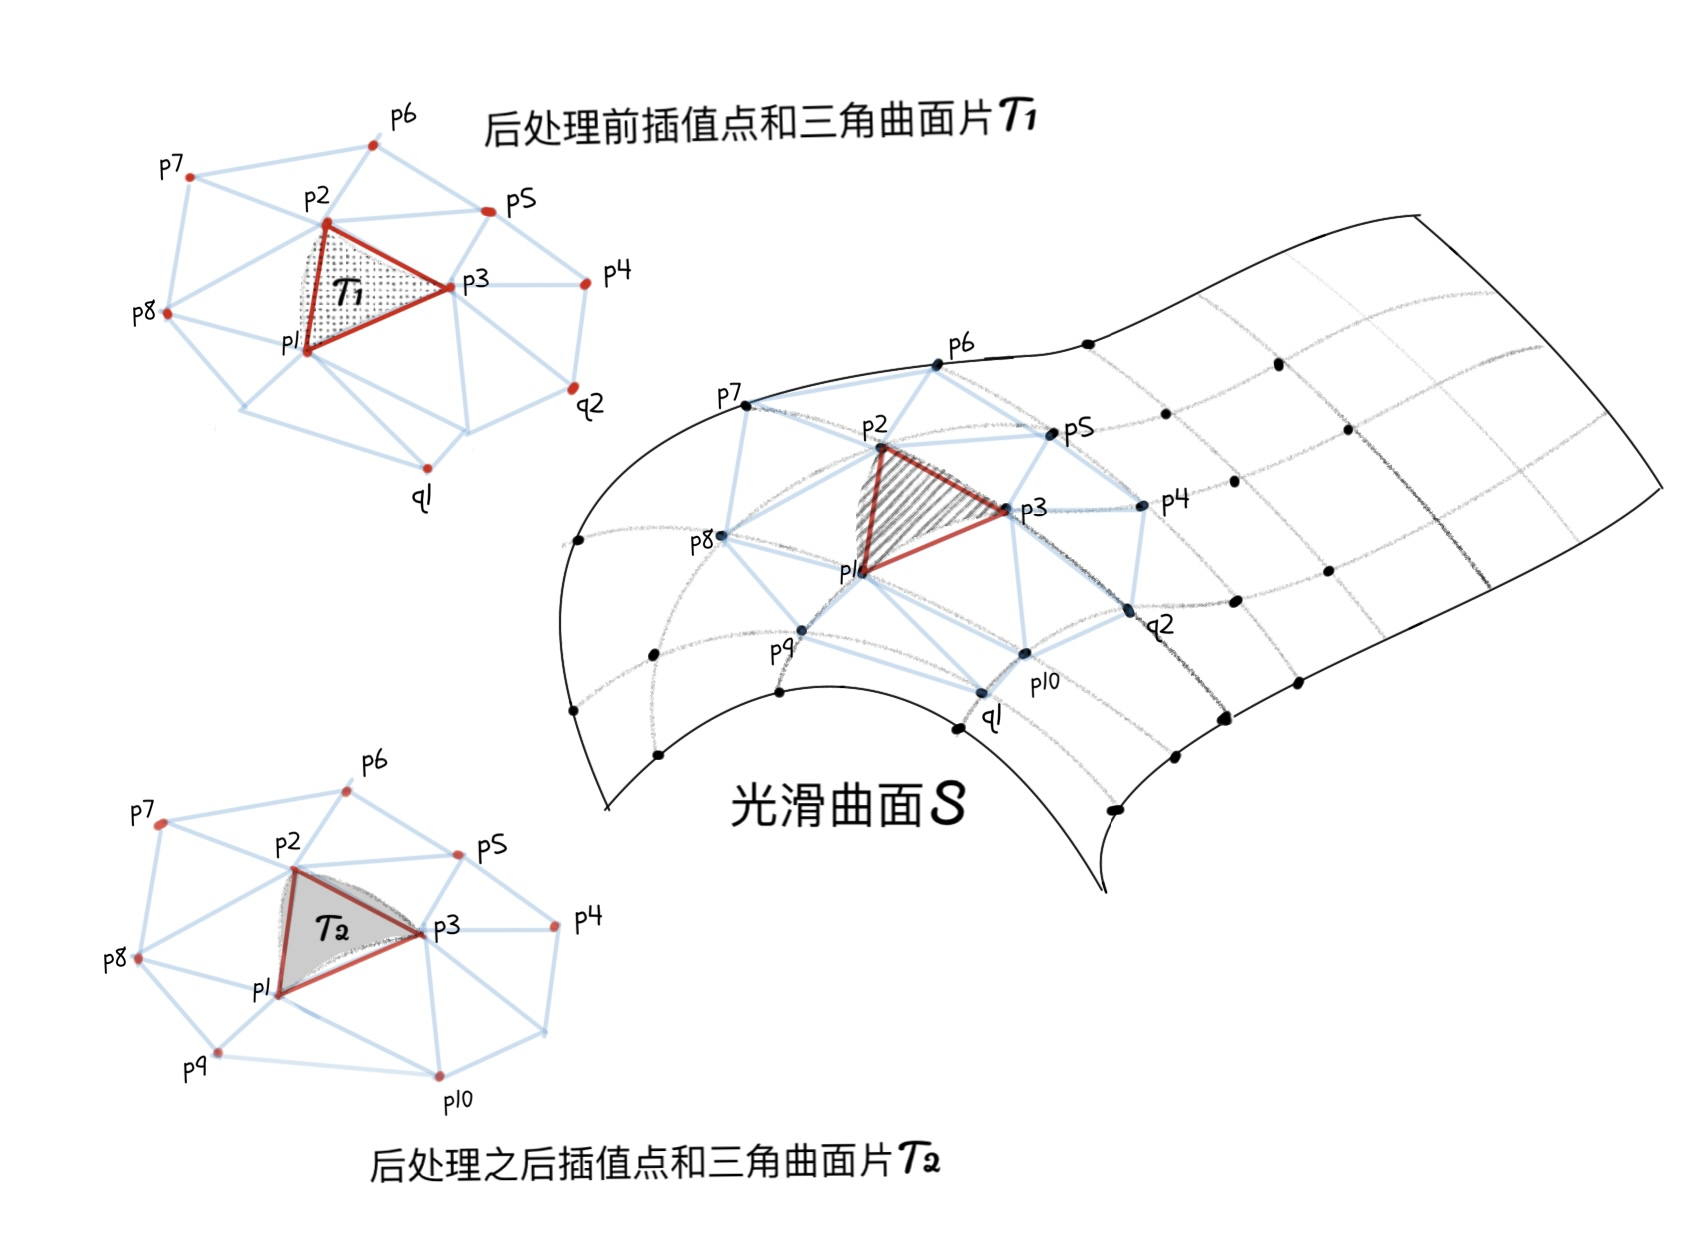
\includegraphics[width=0.7\linewidth]{fig/share}
    \label{fig:share}
  \end{figure}
 后处理算子把靠的太近的点去掉,
 在对应的三角形上用$t_{n+1}$时刻更新的三角剖分中的
 距离三角形重心最近的样本点组插值。
 考虑经过$t_{n+1}$时刻所有的示踪点的一个光滑曲面${\cal S}$.
 由插值的误差精度可知,
 光滑曲面${\cal S}$和
 $\partial\widetilde{{\cal M}}^{n+1}$上对应点的误差是$O(h_L^4)$,
  光滑曲面${\cal S}^{n+1}$和
  $\partial{\cal M}^{n+1}$上对应点的误差也是$O(h_L^4).$
  由积分中值定理得$\left\lVert\widetilde{{\cal M}}^{n+1}\oplus \chi
    \widetilde{{\cal M}}^{n+1}\right\rVert=O(h_L^4)$.
  
令${\cal I}$是恒等映射,
考虑当$k\rightarrow 0,\chi \rightarrow {\cal I},$
所以$\left\lVert\widetilde{{\cal M}}^{n+1}\oplus \chi
    \widetilde{{\cal M}}^{n+1}\right\rVert=0$.
  因此后处理误差也和时间步长$k$相关,
  下面证明误差可以被进一步提高到$O(kh_L^4).$
  
  在$t_{n+1}$时刻,
  考虑三角剖分$\triangle$的一个三角形$T$.
  设$\chi$作用之前的曲面$\widetilde{{\cal M}}^{n+1}$
  上对应三角形$T$的插值或最小二乘拟合得到的近似曲面
   $\vec{f}(\mathbf{x})=\sum_{i=1}^{N}
   (\sum_{j=1}^{M}b_{ij}\varphi^k_{t_n}(p_j))B_i(\mathbf{x});$
    设$\chi$作用后的曲面${\cal M}^{n+1}$
  上对应三角形$T$的插值或最小二乘拟合得到的近似曲面
   $\vec{g}(\mathbf{x})=\sum_{i=1}^{N}
   (\sum_{j=1}^{M}a_{ij}\varphi^k_{t_n}(q_j))B_i(\mathbf{x})$,
   其中
   $\{\varphi^k_{t_n}(q_j)\}_{j=1}^M$是后处理算子作用后的曲面拟合样本点。
   设$p_0,q_0$分别是曲面$\widetilde{{\cal M}}^{n+1},
   {\cal M}^{n+1}$上的一点,
   且$p_0,q_0$在三角形$T$上重心坐标相同。
  
  考虑$t_n$时刻过所有示踪点的光滑曲面${\cal S}^n,$
  ${\cal S}^n$上点$o$在$t_n$时刻三角形$T$上对应坐标和$p_0,q_0$相同。
  易知,
  存在光滑同胚$h^1(t,\mathbf{x}),0\leq t\leq k$, 且
  \begin{displaymath}
  h^1(0)={\cal S}^{n},h^1(k)={\cal S}_1^{n+1},
  h^1(k,\mathbf{x}(o))=p_0, h^1(0,\mathbf{x}(p_j))=p_j,
  h^1(k,\mathbf{x}(p_j))=\varphi^k_{t_n}(p_j),1\leq j\leq M;
\end{displaymath}
 光滑同胚$h^2(t,\mathbf{x}),0\leq t\leq k$, 且
  \begin{displaymath}
  h^2(0)={\cal S}^{n},h^2(k)={\cal S}_2^{n+1},
  h^2(k,\mathbf{x}(o))=q_0, h^2(0,\mathbf{x}(q_j))=q_j,
  h^2(k,\mathbf{x}(q_j))=\varphi^k_{t_n}(q_j),1\leq j\leq M.
\end{displaymath}
由插值唯一性或者拟合多项式对约束条件唯一,有
\begin{displaymath}
  \vec{f}(p)=\sum_{i=1}^{N}\tilde{c}_iB_i(p);\quad
  \vec{g}(p)=\sum_{i=1}^{N}\tilde{d}_iB_i(p),
\end{displaymath}
其中$\{\tilde{c}_i\}$是对$p_0,\{\varphi^k_{t_n}(p_j)\}_{j=1}^{M-1}$
的拟合曲面基函数系数,
$\{\tilde{d}_i\}$是对$p_0,\{\varphi^k_{t_n}(q_j)\}_{j=1}^{M-1}$
的拟合曲面基函数系数。

 设$c_i$是$t_n$时刻对
  $o,p_1,\ldots,p_{M-1}$
  插值或拟合的三次曲面的基函数系数;
  $d_i$是$t_n$时刻对
  $o,q_1,\ldots,q_{M-1}$
  插值或拟合的三次曲面的基函数系数。
  那么,$o=\sum_{i=0}^{M-1}c_iB_i(o)=\sum_{i=0}^{M-1}d_iB_i(o).$
  类似引理\ref{lem:maperror}中对式子(\ref{eq:k})的证明过程,
  用光滑映射$h^1(k,\mathbf{x}(p)),h^2(k,\mathbf{x}(p))$
  代替流映射$\phi_{t_n}^{t_n+k}(p)$,有
  \begin{displaymath}
    \vec{f}(p_0)-o=\sum_{i=1}^{N}\tilde{c}_iB_i(p_0)
    -\sum_{i=0}^{M-1}c_iB_i(o)=O(k);
    \quad \vec{g}(q_0)-o=\sum_{i=1}^{N}\tilde{d}_iB_i(q_0)
   -\sum_{i=0}^{M-1}d_iB_i(o) =O(k).
  \end{displaymath}
  因此有$\lVert p_0-q_0\rVert=O(k),$
  误差精度被提高到$\lVert p_0-q_0\rVert=O(kh_L^4),$
  即$\left\lVert\widetilde{{\cal M}}^{n+1}\oplus \chi
    \widetilde{{\cal M}}^{n+1}\right\rVert=O(kh_L^4)$.

所以
\begin{equation}
  E^{\textmd{ADJ}}(t_n)\leq c_k\sum_{j=1}^{n}\left\lVert
    {\cal E}^\textmd{ADJ}_{j-1}\right \rVert=O(h_L^4).
\end{equation}
\end{pro}


\subsubsection{表示误差$E^\textmd{REP}$、预处理误差$E^\textmd{AUG}$
  和时间积分误差$E^\textmd{ODE}$}
\label{sec:rep,aug,ode}
\begin{prop}
  若半离散映射$\mathring{\phi}$是$\kappa$阶精度的,那么
  $E^{\textmd{ODE}}(t_n)=O(k^\kappa).$
\end{prop}
\begin{pro}
  见推论4.8[MARS]\cite{zhang2016mars}.
\end{pro}

\begin{prop}
  $E^{\textmd{AUG}}(t_n)=0.$
\end{prop}
\begin{pro}
  由算法定义,减去示踪点不改变曲面表示。
\end{pro}


\begin{prop}\label{prop:errorREP}
  任何MARS方法,
  如果用算法\ref{defn:algorithm}中构造的$\mathbb{S}^3_4(\triangle)$曲面
  表示至少$C^4$连续的初始界面,
  也就是${\cal M}^0\in \mathbb{S}^3_4(\triangle)$,
  那么$ E^{REP}(t_n)=O(h_L^4)$.
\end{prop}

\begin{pro}
  对于任意一个三角剖分$\triangle$中的三角形$T$,
  三角形内部任意点对应样条函数上点和初始曲面对应点距离差$O(h_L^4)$.
  对三角形边界上任意点,把点看做原来二元插值三次样条上点,
  插值曲面上近似点和初始点距离差$O(h_L^4).$
  那么三角形对应的局部体积差是$O(h_L^6).$
  
  \begin{figure}[H]
    \centering
    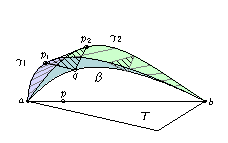
\includegraphics[width=0.35\linewidth]{tikz/volume}
    \label{fig:volume}
  \end{figure}  
  考虑三角曲面片连接处的体积。
  考虑三角剖分三角形边$\overline{ab}$对应参数$s\in[0,1]$,
  线段上一点$p=(1-s)a+sb$,
  对应两个曲面片边界上点$p_1,p_2$,初始曲面上点$q$
  两个曲面片边界表示$\gamma_1(s),\gamma_2(s)$,
  初始曲面对应曲线$\beta(s)$.
  对所有参数$s$,
  直线段连接三个点,
  组成体积的边界。
  $\beta(s)$上点$q$两个曲面片$\gamma_1(s),\gamma_2(s)$上点$p_1,p_2$,
  组成体积的三角形横截面。
  三角形$\triangle_{qp_1p_2}$的面积是$O(h_L^8)$的,
  则局部连接处体积$O(h_L^9)$.
  又因为所有的三角剖分中三角形个数是$O(\frac{1}{h_L^2})$,
  则所有连接处体积和是$O(h_L^7)$,
  那么
  \begin{displaymath}
    E^{REP}(t_n)=\lVert \phi^{nk}_{t_0}({\cal M}(t_0))\oplus
  \phi^{nk}_{t_0}({\cal M})\rVert
  =\lVert {\cal M}(t_0)\oplus{\cal M}^0\rVert(1+O(kn))
  =O(h_L^6)O(\frac{1}{h_L^2})+O(h_L^7)=O(h_L^4).
  \end{displaymath}
\end{pro}

%%% Local Variables:
%%% mode: latex
%%% TeX-master: t
%%% End:


\section{局部多项式曲面构造}
% \noindent{\parbox{\textwidth}{{\wn{Question:}
%       几阶的多项式曲面可以使得界面追踪精度达到4阶?}}}
% \noindent{\fbox{\parbox{\textwidth}{{\wn{Question:}
%        几阶的多项式曲面可以使得界面追踪精度达到4阶?
%        \uline{u*}}}}}
 % \begin{itemize}
 % \item 推广一元多项式插值余项的推导方式?
 %   ($\mathrm{R}^m\rightarrow \mathrm{R}^n的Roller's Theorem$)
 % \item 参考张量曲面的误差分析
 % \item 转化成点在曲线上分析?
 % \end{itemize}
\begin{rem}
  由于我们用于追踪流体界面的点在空间上是散乱分布的,
  而且已经有三角剖分的结构,因此我们考虑基于三角剖分的二维样条函数。
\end{rem}
\subsection{Bernstein 基多项式}
%%%%%%%%%%%%%%%%%%%%%%%%%%%%% Constants
% a.向前追踪边界上的示踪点b.如果下一时刻的三角性边长大于$h_L$,
% 回溯原来的三角形,在原来的三角形边长中增加中点对应的插值曲面上的点作为新的示踪点

%  插值曲面的构造。

% 将三角网格点投影在x-y平面,向外找star上的示踪点投影到x-y平面。
% 如果一层star没有合适的十个点就向外再裹一层。

% 取最外面的三个点构成包裹的三角形T,
% 运用三角形的重心坐标和Bernstein basis polynomials of degree d relative
% to T,
\begin{nota}
  $d$阶多项式空间
  \begin{displaymath}
{\cal P}_d:=\left\{ p(x,y) = \sum_{0\leq i+j\leq d}c_{ij}x^iy^j\right\}.
  \end{displaymath}
\end{nota}
\begin{defn}
  给定整数$d>0$,和三角形$T$相关的$d$阶 Bernstein 基多项式定义为
  \begin{displaymath}
    B^d_{ijk}:=\frac{d!}{i!j!k!}b^i_1b_2^jb_3^k,\quad i+j+k=d,
  \end{displaymath}
  $i,j,k$是非负整数。
\end{defn}
\begin{prop}
  Bernstein基多项式性质:
  \begin{enumerate}
  \item $ 0\leq B_{ijk}^d(x,y)\leq 1 \quad (x,y) \in T,$
  \item $ \sum_{i+j+k=d}B_{ijk}^d(x,y) \equiv 1\quad (x,y)\in T.$
  \end{enumerate}
\end{prop}


\begin{lem}
  多项式 $\left\{ B^d_{ijk}\right\}$线性独立,
  且构成$d$次多项式${\cal P}_d$线性空间的一组基,维数是
  $\begin{pmatrix}
    d+2\\ 2
  \end{pmatrix}$。
\end{lem}

% \begin{nota}
%   ${\cal S}^0_d(\triangle):=\{s\in C^0(\Omega):s|_{T_i}\in{\cal P}_d ,
%   \quad i=1,...,n_t\}.$
% \end{nota}
% \begin{prop}  \begin{displaymath}
% \textmd{dim} {\cal S}^0_d(\triangle)=n_v+(d-1)n_e+\frac{(d-1)(d-2)}{2}n_t,
% \end{displaymath}
% 其中,$n_v,n_e$和$n_t$分别是三角剖分的点、边和三角形个数。
% \end{prop}

\begin{rem}
  为了达到四阶精度,我们用$p\in {\cal P}_3$
  \begin{displaymath}
    p(x,y)=\sum_{i+j+k=3}c_{ijk}B_{ijk}^d=\sum_{i=1}^{10}c_iB_i,
  \end{displaymath}
  其中$c_i,1\leq i\leq 10$分别
  是
  $c_{300},c_{210},c_{201},c_{120},c_{111},c_{102},c_{030},c_{021},c_{012}$,
  $c_{003}$.
\end{rem}



\begin{rem}
  考虑以下两种局部曲面表示
  \begin{enumerate}
  \item 基于适定结点组生成算法的局部二元三次多项式插值\cite{ShaoThesis};
  \item 基于三角剖分的局部部分插值部分最小二乘拟合
    \cite{schumaker2015spline}.
  \end{enumerate}
\end{rem}

\subsection{基于三角剖分的局部部分插值部分最小二乘拟合}
\label{sec:局部三次样条曲面}
\begin{defn}[算法]\cite{schumaker2015spline}
  对于任意的三角剖分中的三角形,
\begin{enumerate}
\item 以三角形为中心,寻找合适的拟合点。
  取三个顶点star中的所有点。
  如果点大于20,取距离三角形中心最近的20个点。
\item 根据在三个三角形顶点插值,最小二乘拟合其他点的条件,
  计算三次样条基函数的系数。
\end{enumerate}
\end{defn}

\begin{lem}
  设三角形$T$ 的三个顶点分别是$v_1,v_2$ 和 $v_3$.
 给定点列 $\{p:=(x_i,y_i)^m_{i=1}\}$对应的值 $\{z_i\}^m_{i=1}$
 令
  \begin{displaymath}
    O:=[B_1(p_j),...,B_{10}(p_j)]_{j=1}^m,
  \end{displaymath}
  其中$B_1,...,B_{10}$是关于$T$的三次Bernstein基多项式。
  令$\tilde{O}$是$O$去掉第1,7,10列的子矩阵,且满秩。
  则对任意的$\{\omega_i\}_{i=1}^3$,存在一个唯一的二元三次多项式使得
  \begin{displaymath}
    g:=\sum_{i=1}^{10}c_iB_i
  \end{displaymath}
  满足$g(v_i)=w_i,i=1,2,3$,且极小化
  \begin{displaymath}
    \sum_{j=1}^m[g(p_j)-z_j]^2.
  \end{displaymath}
\end{lem}

\begin{pro}
  由Bernstein基多项式的性质可以通过令$c_1 = w_1, c_7 = w_2, c_{10} = w_3$确保$g(v_i)=w_i,i=1,2,3$。
  \begin{displaymath}
    \boldsymbol{c} = \left[
      \begin{matrix}
        c_2\\
        \vdots\\
        c_6\\
        c_8\\
        c_9
      \end{matrix}
    \right], 
    \boldsymbol{b} = \left[
      \begin{matrix}
        z_1\\
        \vdots\\
        z_m
      \end{matrix}
    \right] - w_1O_1-w_2O_7-w_3O_{10}.      
  \end{displaymath}
  为了得到其余的多项式,求解超定方程组
  \begin{displaymath}
    \tilde{O}\boldsymbol{c} = \boldsymbol{b}
  \end{displaymath}
  由于$\tilde{O}$列满秩,等价于求解正规方程
  \begin{displaymath}
    \tilde{O}^T\tilde{O}\boldsymbol{c} = \tilde{O}^T\boldsymbol{b}.
  \end{displaymath}
  得到唯一的最小二乘解。
\end{pro}

\subsection{数值测试结果}

\begin{figure}[H]
  \centering
  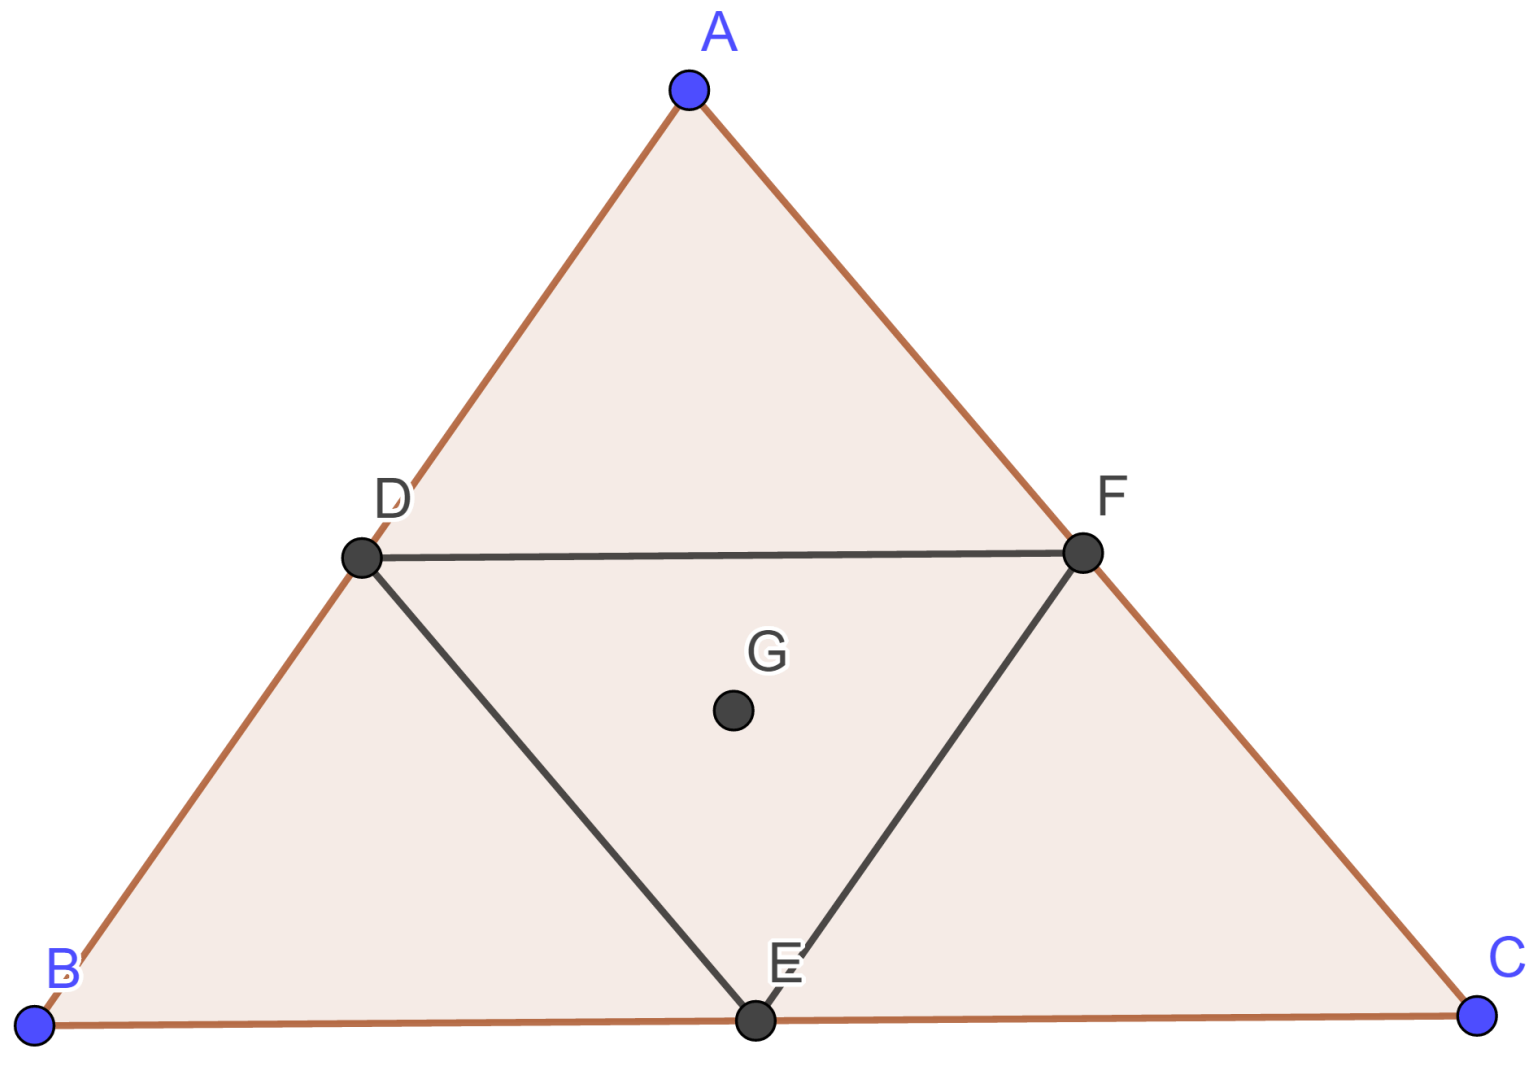
\includegraphics[width=0.35\linewidth]{images/tri}
  \caption{加密网格的方法}
\end{figure}
\begin{table}[htbp]
  \begin{center}  
    \begin{tabular}{|l|l|l|l|l|l|l|l|}  
      \hline  
      norm & $|E_h|$ & rate & $|E_{h/2}|$ & rate& $|E_{h/4}|$ &rate &$|E_{h/8}|$ \\
      \hline            
      1-norm & 2.77e-3 & 3.09 & 3.25e-4 & 4.34& 1.60e-5 & 3.89&1.07e-6 \\
      \hline
      2-norm & 5.97e-4 & 3.56 & 5.05e-5 & 4.00& 3.15e-6 & 4.82&1.11e-7 \\
      % 5 & 2.11e-3 & 8.12 & 3.28e-3 & -& 9.88e-06 \\  \hline
      \hline  
    \end{tabular}  
  \end{center}  
  \caption{局部完全插值}  
\end{table}
\begin{table}[h]
  \centering
  \begin{tabular}{|c|c|c|c|c|c|c|}
    \hline
    $|E_h|$ & rate & $|E_{h/2}|$ & rate& $|E_{h/4}|$&rate&$|E_{h/8}|$\\ 
    \hline
    1.74e-5& 5.19& 4.77e-7& 5.10& 1.38e-8& 4.03& 8.48e-10\\ 
    \hline
  \end{tabular}
  \caption{局部部分插值结合最小二乘}
\end{table}



\input{sec/ref}
%\end{CJK*}
\end{document}

%%% Local Variables:
%%% mode: latex
%%% TeX-master: t
%%% End:
